\documentclass{jsarticle}

\usepackage{amsmath}
\usepackage{amssymb}
\usepackage{booktabs}
\usepackage{float}
\usepackage{graphicx}
\usepackage{listings}
\usepackage{url}
\usepackage{subcaption}

\lstset{
  basicstyle={\ttfamily},
  identifierstyle={\small},
  commentstyle={\smallitshape},
  keywordstyle={\small\bfseries},
  ndkeywordstyle={\small},
  stringstyle={\small\ttfamily},
  frame={tb},
  breaklines=true,
  columns=[l]{fullflexible},
  numbers=left,
  xrightmargin=0zw,
  xleftmargin=3zw,
  numberstyle={\scriptsize},
  stepnumber=1,
  numbersep=1zw,
  lineskip=-0.5ex
}

\title{情報領域演習第二 L演習(クラス3) レポート}
\author{学籍番号: 1810678 \\
        名前: 山田朔也}

\begin{document}
    \maketitle
    \begin{description}
        \item[問1.]
        \begin{description}
            \item[(a)]
            作成した状態は以下の図\ref{fig1}のようになった。また、状態遷移図がこのようになる理由は問1の(b)にて説明する
            \begin{figure}[H]
                \centering
                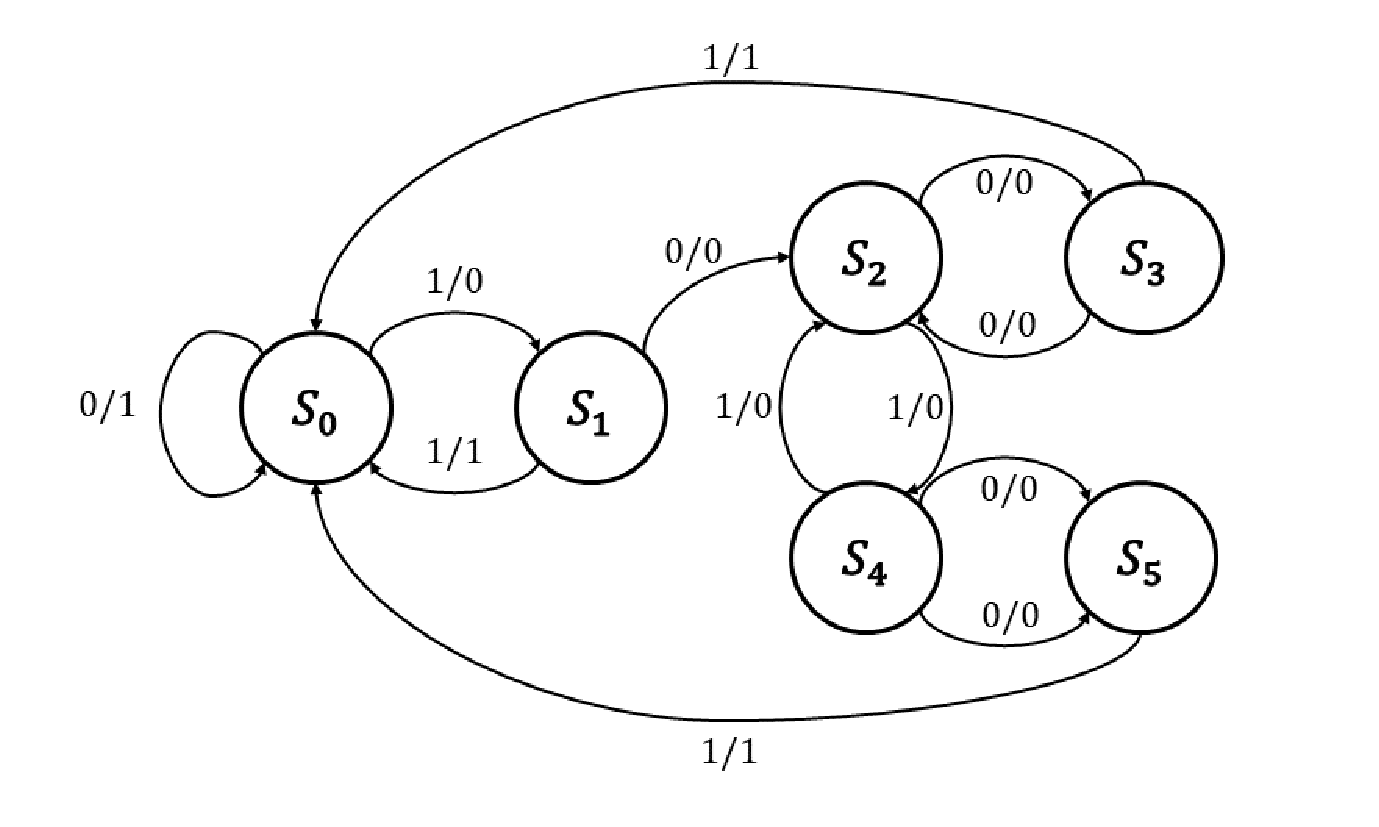
\includegraphics[width = 10cm]{fig_1.eps}
                \caption{最上位ビットから読み取った時の状態遷移図}
                \label{fig1}
            \end{figure}

            \item[(b)]
            (a)で作成した状態遷移図の状態遷移表は以下の表\ref{tab1}のようになる。
            \begin{table}[H]
                \centering
                \caption{状態遷移図\ref{fig1}の状態遷移表}
                \label{tab1}
                \begin{tabular}{|c|c|c|} \hline
                    & 0 & 1 \\ \hline
                    $S_0$ & $S_0 \,,\, 1$ & $S_1 \,,\, 0$ \\ \hline
                    $S_1$ & $S_2 \,,\, 0$ & $S_0 \,,\, 1$ \\ \hline
                    $S_2$ & $S_3 \,,\, 0$ & $S_4 \,,\, 0$ \\ \hline
                    $S_3$ & $S_2 \,,\, 0$ & $S_0 \,,\, 1$ \\ \hline
                    $S_4$ & $S_5 \,,\, 0$ & $S_2 \,,\, 0$ \\ \hline
                    $S_5$ & $S_4 \,,\, 0$ & $S_0 \,,\, 1$ \\ \hline
                \end{tabular}
            \end{table}

            ここからこの状態遷移表を講義で習ったように、等価な状態でグループ分けをしてしていくと以下の表\ref{tab2}のようになった。
            \begin{table}[H]
                \centering
                \caption{グループ分けの遷移}
                \label{tab2}
                \begin{tabular}{|c|c|c|c|} \hline
                    & 現状態 & 0 & 1 \\ \hline
                    $B_0^1$ & $S_0$ & $B_0^1$ & $B_1^1$ \\ \hline
                    $B_1^1$ & $S_1$ & $B_2^1$ & $B_0^1$ \\ \cline{2-4}
                     & $S_3$ & $B_2^1$ & $B_0^1$ \\ \cline{2-4}
                     & $S_5$ & $B_2^1$ & $B_0^1$ \\ \hline
                    $B_2^1$ & $S_2$ & $B_1^1$ & $B_2^1$ \\ \cline{2-4}
                     & $S_4$ & $B_1^1$ & $B_2^1$ \\ \hline
                \end{tabular}
            \end{table}

            これより、簡単化ができる。そして、簡単化後の状態遷移表と、その符号化を行った状態遷移表は以下の表\ref{tab3},\ref{tab4}のようになる。
            \begin{table}[H]
                \centering
                \begin{minipage}{0.4\columnwidth}
                    \centering
                    \caption{簡単化後の状態遷移表}
                    \label{tab3}
                    \begin{tabular}{|c|c|c|} \hline
                        & 0 & 1 \\ \hline
                        $S_0^*$ & $S_0^* \,,\, 1$ & $S_1^* \,,\, 0$ \\ \hline
                        $S_1^*$ & $S_2^* \,,\, 0$ & $S_0^* \,,\, 1$ \\ \hline
                        $S_2^*$ & $S_1^* \,,\, 0$ & $S_2^* \,,\, 0$ \\ \hline
                    \end{tabular}
                \end{minipage}
                \begin{minipage}{0.4\columnwidth}
                    \centering
                    \caption{符号化後の状態遷移表}
                    \label{tab4}
                    \begin{tabular}{|c|c|c|} \hline
                        & 0 & 1 \\ \hline
                        00 & $00 \,,\, 1$ & $01 \,,\, 0$ \\ \hline
                        01 & $10 \,,\, 0$ & $00 \,,\, 1$ \\ \hline
                        10 & $01 \,,\, 0$ & $10 \,,\, 0$ \\ \hline
                    \end{tabular}
                \end{minipage}
            \end{table}

            ここから論理式を求めていく。まず、符号化した状態の0,1の列において下位ビットを$s_0$,上位ビットを$s_1$とする。
            また、入力は$x$,出力を$f$とすると、$s_0 \,,\, s_1 \,,\, f$のカルノー図は以下の図\ref{fig2}のようになる。
            \begin{figure}[H]
                \centering
                \begin{subfigure}{0.2\columnwidth}
                    \centering
                    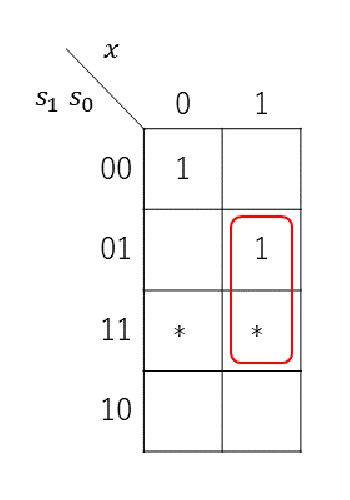
\includegraphics[width=\columnwidth]{fig_2_f.eps}
                    \caption{$f$のカルノー図}
                    \label{fig2_f}
                \end{subfigure}
                \begin{subfigure}{0.2\columnwidth}
                    \centering
                    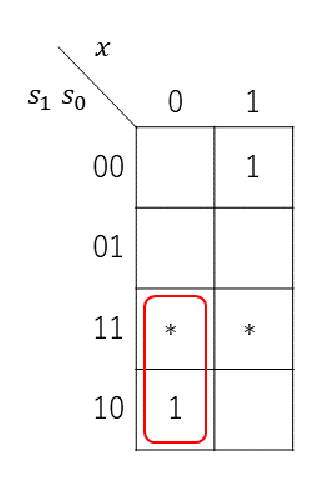
\includegraphics[width=\columnwidth]{fig_2_s0.eps}
                    \caption{$s_0$のカルノー図}
                    \label{fig2_s0}
                \end{subfigure}
                \begin{subfigure}{0.2\columnwidth}
                    \centering
                    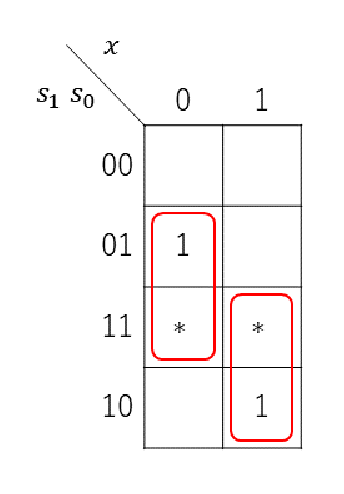
\includegraphics[width=\columnwidth]{fig_2_s1.eps}
                    \caption{$s_1$のカルノー図}
                    \label{fig2_s1}
                \end{subfigure}
                \caption{カルノー図}
                \label{fig2}
            \end{figure}

            次にこれらのカルノー図から論理式を作成すると以下のようになる。
            \begin{align}
                f &= \overline{x s_0 s_1} + xs_0 \\
                s_0 &= \overline{x}s_1 + x\overline{s_0 s_1} \\
                s_1 &= \overline{x}s_0 + xs_1
            \end{align}

            これを回路化したものが以下の図\ref{fig3}となる。
            \begin{figure}[H]
                \centering
                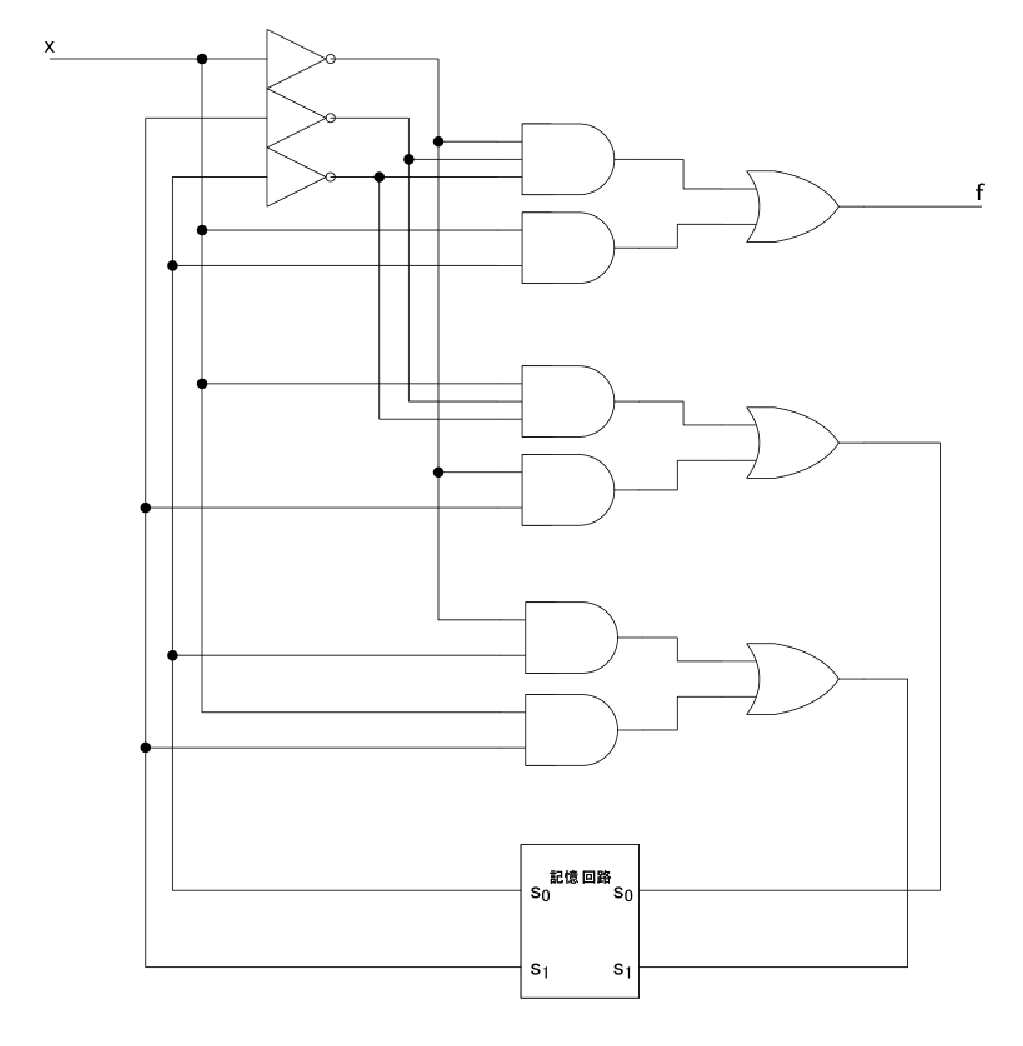
\includegraphics[width=10cm]{fig_3.eps}
                \caption{作成された回路図}
                \label{fig3}
            \end{figure}

            \item[(c)]
            まず、最初に考えるのは2進数において各ビットが1になった場合に増える値は$\pmod 3$における値である。
            これは以下のようになる。
            \begin{align}
                \cdots \,1\,2\,1\,2\,1\,2\, \cdots
            \end{align}
            ここから、$n$が3の倍数となるためには「間が奇数個離れた1となっているビットが3つ存在する」もしくは「2つの1となっているビットの間が偶数個離れている、もしくは隣り合っている」
            という条件を$n$が満たしている必要がある。
            これらを満たすように設計したものが(a)で記述した図\ref{fig1}である。この回路はその状態遷移図を簡単化したものであるため、正しく動作することが分かる。
        \end{description}

        \item[問2.]
        \begin{description}
            \item[(a)]
            アルゴリズム自体は問1と全く同一のものを用いて計算することとなる。
            また、今回は簡単化の手間を省くため、問1で簡単化された後の状態遷移表を用いて状態遷移図書いていくこととする。
            実際に書いた状態遷移図は以下の図\ref{fig4}のようになった。
            \begin{figure}[H]
                \centering
                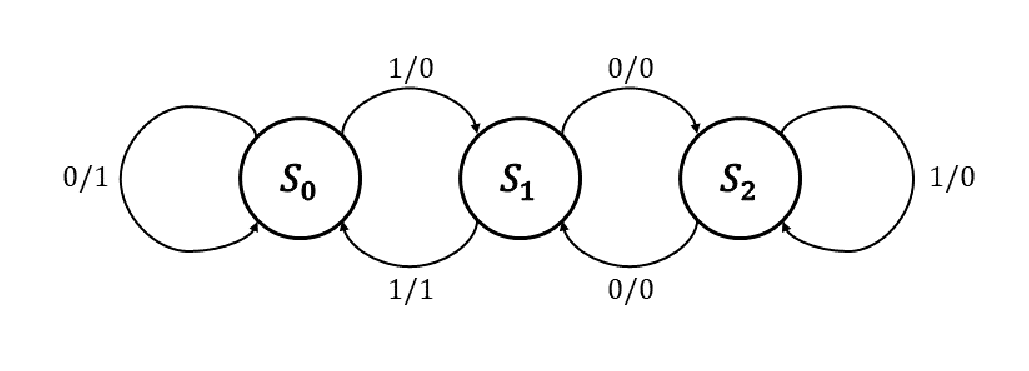
\includegraphics[width = 10cm]{fig_4.eps}
                \caption{最上位ビットから読み取った時の状態遷移図}
                \label{fig4}
            \end{figure}

            \item[(b)]
            この回路は問1.の(b)の図\ref{fig3}と同一である。

            \item[(c)]
            これも問1と同様であるため問1の(c)と同一の理由である。
        \end{description}

        \item[問3.]
        分かりませんでした。ただ、$n$の$pmod 3$は3通りに分けられることに関係があるのでは無いかと思いました。

        \item[問4.]
        \begin{description}
            \item[(a)]
            まずこの文字列の受け取り方から考えていく。今回は特に指定がなかったため、
            文字列の最初の文字と最後の文字それぞれから中央に向かって一つずつずらしながら入力していく。
            そのため入力数は2つとなる。では実際の状態遷移図がどのようになるかというと、のカルノー図は以下の図\ref{fig5}のようになった。
            \begin{figure}[H]
                \centering
                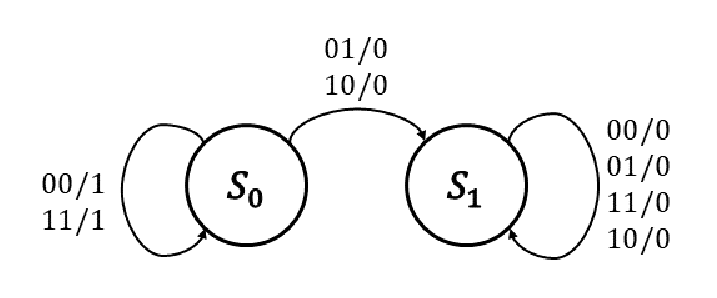
\includegraphics[width=6cm]{fig_5.eps}
                \caption{回文か否かを判定する状態遷移図}
                \label{fig5}
            \end{figure}
            また、この図内での入力が暫定的に0,1で表されている。
            なぜなら順序回路化するにあたって符号化することを考えると0,1上での文字列を考えれば十分であるからである。

            \item[(b)]
            (a)で作成した状態遷移図の状態遷移表は以下の表\ref{tab5}のようになる。
            また、$S_0$を0,$S_1$を1として符号化したものを掲載している。
            \begin{table}[H]
                \centering
                \caption{回文か否かを判定する状態遷移表}
                \label{tab5}
                \begin{tabular}{|c|c|c|c|c|} \hline
                     & 00 & 01 & 10 & 11 \\ \hline
                    0 & 0,1 & 1,0 & 1,0 & 0,1 \\ \hline
                    1 & 1,0 & 1,0 & 1,0 & 1,0 \\ \hline
                \end{tabular}
            \end{table}
            また、これはこれ以上簡易化することはできない。
            そして、これの入力を$x,\, y$、出力を$f$、状態を$s$とすると以下の図\ref{fig6}ようなカルノー図を書くことができる。
            \begin{figure}[H]
                \centering
                \begin{subfigure}{0.2\columnwidth}
                    \centering
                    \includegraphics[width=\columnwidth]{fig_6_f.eps}
                    \caption{$f$のカルノー図}
                    \label{fig6_f}
                \end{subfigure}
                \begin{subfigure}{0.2\columnwidth}
                    \centering
                    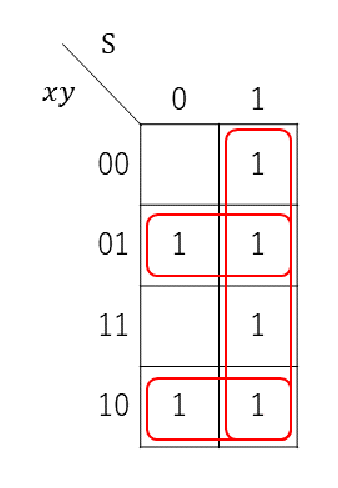
\includegraphics[width=\columnwidth]{fig_6_s.eps}
                    \caption{$s$のカルノー図}
                    \label{fig6_s}
                \end{subfigure}
                \caption{カルノー図}
                \label{fig6}
            \end{figure}

            次にこれらのカルノー図から論理式を作成すると以下のようになる。
            \begin{align}
                f &= \overline{x y s} + xy\overline{s} \\
                s &= s + \overline{x}y + x\overline{y}
            \end{align}

            これを回路化したものが以下の図\ref{fig7}となる。
            \begin{figure}[H]
                \centering
                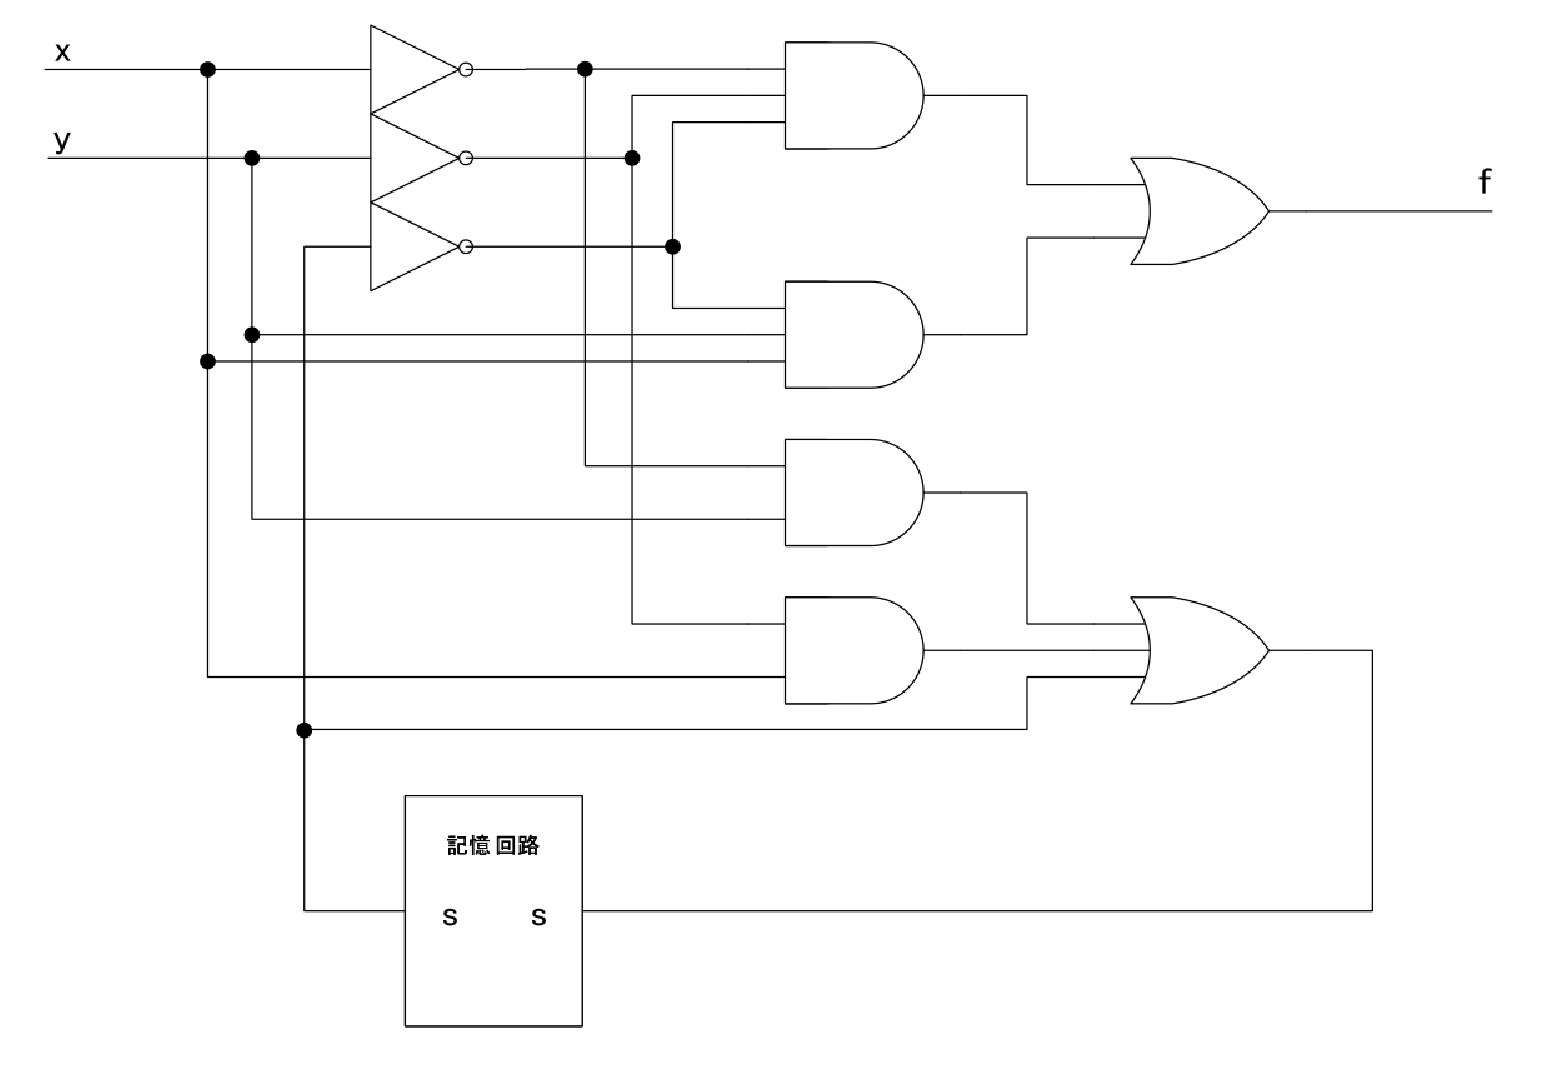
\includegraphics[width=10cm]{fig_7.eps}
                \caption{作成された回路図}
                \label{fig7}
            \end{figure}

            \item[(c)]
            入力文字列の長さの制限を取り払う、それはつまり文字列の長さが定義されず、文字列の終わりが無いということとなる。
            回文において、終わりの無い文字列というのは存在しない。なぜならば回文は少なくとも文字列の初めと終わりが一致していなくていけない。
            しかし、文字列に終わりがなければこれを満たすことはないからである。
            \\
            また、文字列を少なくとも半分は記憶しておかなくては回分か否か判断できないため、文字列が無限であれば記憶装置の容量も無限で無くてはならない。

        \end{description}
    \end{description}
\end{document}
